\begin{frame}{Файловая система.}
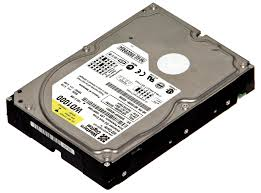
\includegraphics[height=4cm]{hw_hdd.jpg} 
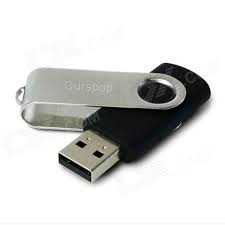
\includegraphics[height=4cm]{hw_usb_stick.jpg} 
  \begin{itemize}
    \item Hardware (HDD, Disk controllers, SAS, SCSI, SATA)
    \item Drivers, block devices (disks or partitions)
    \item File system (NTFS, FAT, ext4, xfs)
  \end{itemize}
\end{frame}

\begin{frame}{Базовые определения}
  \begin{itemize}
    \item В UNIX (и Linux) файлы организованы в виде \emph{единой древовидной структуры} (дерева), называемой \alert{файловой системой}.
    \item Корнем дерева является \alert{корневой каталог} (root directory), имеющий имя \alert{"/"}.
    \item \alert{root file system} - блочное устройство, которое содержит файлы для работы операционной системы и монтируется в /
    \item \alert{монтирование} - процесс отображения содержимого устройства в указанную директорию файловой системы.
  \end{itemize}
\end{frame}
\begin{frame}{Графической представление файлового дерева}
      \begin{block}{Упражнение. Найдите на рисунке:}
	      Корневой каталог.  На каком устройстве находится root file system?
	      Точки монтирования блочных устройств.
      \end{block}
  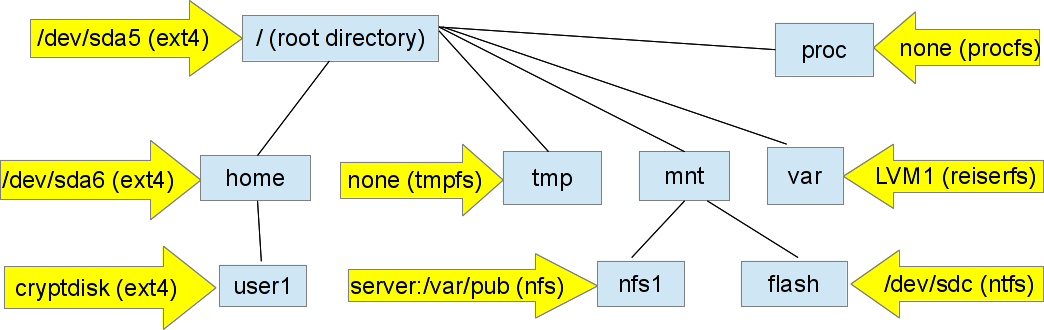
\includegraphics[height=3.5cm]{vfs-and-devices}
\end{frame}

\begin{frame}{Команды подключения дисков в файловое дерево}
      \begin{itemize}
        \item монтировать - ( \alert{mount} ) 
        \item размонтировать ( \alert{umount} )
      \end{itemize}
   \alert{mount} без параметров - вывести список уже подключенных файловых систем
      \begin{block}{Упражнение. Дерево монтирования.}
     Получить вывод смонтированных блочных устройств в виде дерева с помощью команды: \alert{findmnt}
      \end{block}
\end{frame}

